\chapter{Datenverarbeitung}
\label{ch:data_processing}

\section{Herkömmliches Analysevorgehen}
\label{sec:common_analysis_approach_part2}

In Kapitel \ref{sec:common_analysis_approach_part1} wurde bereits besprochen, wie bei der Open-Source Software \textit{Autopsy} ein Fall angelegt und Datenträgerabbilder hinzugefügt werden können. Schon bei dem Importieren eine Datenquelle können diverse Module zur automatisierten Datenaufbereitung aktiviert werden. Dies entspricht der dritten Phase, dem \textit{Sichten und Aufbereiten} aus dem allgemeinen forensischen Analyseprozess.\footnote{Siehe Abbildung \ref{fig:digital_forensics_process} In Kapitel \ref{sec:common_analysis_process}.} Diese Module werden nachfolgend beschrieben, um einen Vergleich zur hier entwickelten forensischen Analyseplattform zu ermöglichen.\\
Abbildung \ref{fig:autopsy_2_ingest_modules} zeit die verfügbaren Module.

\begin{figure}[ht]
  \centering
  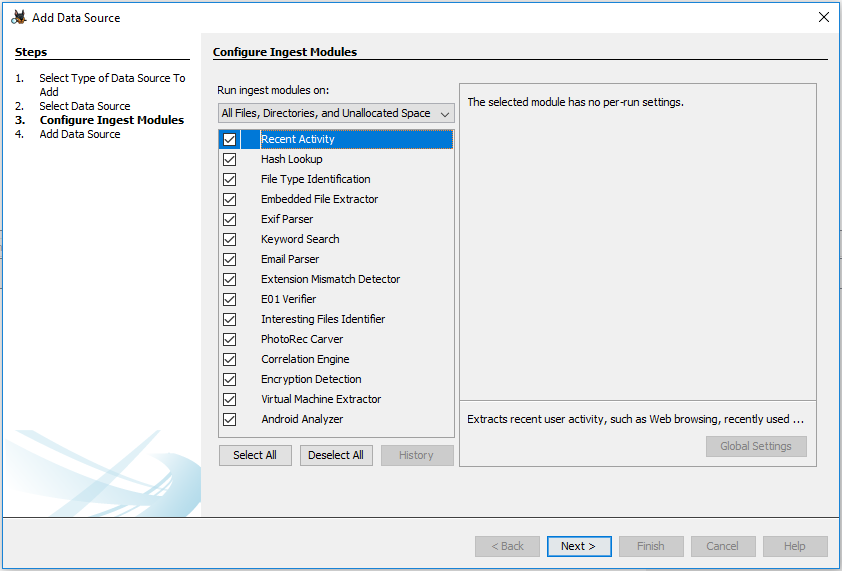
\includegraphics[width=0.78\textwidth]{./resource/autopsy_2_ingest_modules.png}
  \caption{Module zur automatischen Datenverarbeitung bei Autopsy}
  \label{fig:autopsy_2_ingest_modules}
\end{figure}

\noindent
Nachfolgend werden die Module kurz beschrieben und mit der Funktionalität der hier entwickelten forensischen Analyseplattform verglichen. Zuerst werden die Module aufgelistet, welche ganz oder teilweise auch in der forensischen Analyseplattform implementiert sind.\footnote{Siehe Link: \url{http://sleuthkit.org/autopsy/docs/user-docs/4.3/}. Letzter Zugriff: 09.08.2018.}

\begin{itemize}
\item Das \textit{File Type Identification Modul} ermöglicht die Ermittlung von Medientypen und Dateiformaten, wie beispielsweise \textit{JPEG}-Bilder. Autopsy nutzt hier die Open-Source Bibliothek Apache Tika\texttrademark. Ein gleichwertige Funktionalität wird auch auch für die forensische Analyseplattform entwickelt.\footnote{Siehe Kapitel \ref{subsec:media_types}.}
\item Das \textit{Correlation Engine Modul} bietet eine Möglichkeit mehrere Fälle und ihre Datenquellen miteinander zu verknüpfen, um Beziehungen untereinander zu erkennen. Analog hierzu bietet auch die forensische Analyseplattform mit dem Auffinden von Datei-Duplikaten, eine einfache Funktion um Beziehungen zwischen mehreren Fällen und den Asservaten herzustellen.\footnote{Siehe Kapitel \ref{subsec:duplicate_files}}
\item Das \textit{Keyword Search Modul} ermöglicht eine Schlüsselwortsuche. Hierzu werden Dateien mithilfe von Apache Solr indiziert. Darüber hinaus kann mithilfe diverser Regulären Ausdrücken nach bestimmten Strukturen, wie beispielsweise E-Mail- oder Web-Adressen gesucht werden. Die hier entwickelte Analyseplattform implementiert auch eine Textsuche auf Basis von Apache Solr. Derzeit ist es allerdings noch nicht möglich ganze Dateiinhalte zu indexieren.\footnote{Siehe Kapitel \ref{subsec:file_indexing}.}
\end{itemize}

\noindent
Nachfolgend werden die Module von Autopsy aufgelistet, welche noch nicht in der forensischen Analyseplattform vorhanden sind und in Weiterentwicklungen der Plattform implementiert werden könnten.
\begin{itemize}
\item Das \textit{Recent Activity Modul} versucht anhand der Zeitstempel alle interessanten Tätigkeiten der letzten 7 Tage zu ermitteln, wie zum Beispiel besuchte Websites von diversen Browsern.
\item Das \textit{Hash Lookup Modul} ermöglicht es die Datei-Hashsummen mit bereits bekannten Hashsummen zu vergleichen. Damit könnten bekannte Betriebssystemdateien schnell gefiltert werden. Analog zu einem Virenscanner könnte dadurch auch bekannte bösartige Malware gefunden werden.
\item Das \textit{Embedded File Extractor Modul} ermöglicht das Entpacken von Archivdateien, wie beispielsweise \textit{ZIP}-Dateien.
\item Das \textit{Exif Parser Modul} ermöglicht die Anzeige der sogenannten \textit{EXIF}-Metadaten aus \textit{JPEG}-Bilddateien. In der forensischen Analyseplattform könnte diese Funktionalität auch mit Apache Tika implementiert werden.
\item Das \textit{Email Parser Modul} extrahiert E-Mails aus diversen E-Mail Archiven, wie beispielsweise dem \textit{PST}-Dateiformat, welches von Microsoft Outlook genutzt wird.
\item Das \textit{Extension Mismatch Detector Modul} ermittelt Dateien, der Dateiendung nicht zum analysierten Medientyp auf Basis des Dateiinhalts passen. Dies könnte auf versteckte Dateien hinweisen. Ein ähnliche Funktion könnte in der forensischen Analyseplattform über die Volltextsuche implementiert werden, da die Dateiendung und der Medientyp bekannt sind.
\item Das \textit{E01 Verifier Modul} prüft speziell für das forensische Analyseformat \textit{E01} die Dateiprüfsummen mit den gespeicherten Prüfsummen. Damit könnten Änderungen an dem sichergestellten Datenträger ermittelt werden.
\item Das \textit{Interesting Files Identifier Modul} identifiziert interessante Dateien, welche vorher durch bestimmten Suchkriterien, wie beispielsweise Dateinamen und Datentypen, definiert wurden.
\item Das \textit{PhotoRec Carver Modul} ermöglicht das bereits beschriebene File Carving auf ungenutzten Speicherbereichen. Diese Funktionalität wird nicht von der forensischen Analyseplattform unterstützt, da ungenutzte Speicherbereiche aus den originalen Datenträgerabbilder nicht in das Analysesystem importiert werden.
\item Das \textit{Encryption Detection Modul} ermöglicht das Auffinden von verschlüsselten Containern. Hierbei wird nach Dateien gesucht, deren Inhalt eine hohe Entropie aufweisen.\footnote{Die Entropie in der Informationstechnik ist ein Maß zur Bestimmung des mittleren Informationsgehalts pro Zeichen. Bei verschlüsselten Containern ist diese Entropie sehr hoch verglichen zu unverschlüsselten Dateien. TODO: Krypto-Buch als Quelle nutzen...}
\item Das \textit{Virtual Machine Extractor Modul} kann Dateien aus Systemabbildern von virtuellen Maschinen extrahieren.
\item Das \textit{Android Analyzer Modul} ermöglicht das Extrahieren von bestimmten Informationen aus spezifischen Dateien des Android-Betriebssystems. So können beispielsweise Kontaktdaten und Nachrichten aus für Android spezifischen SQLite-Datenbanken ermittelt werden.
\end{itemize}

\noindent
Nachdem die benötigten Module in Autopsy aktiviert und nach fallspezifischen Eigenschaften konfiguriert wurden, erfolgt die Datenaufbereitung im Hintergrund. Parallel hierzu kann der Analyst bereits die Rohdaten analysieren.\footnote{Siehe Kapitel \ref{ch:data_visualization} zur Visualisierung von Daten.}\\

\section{Umsetzung in der forensischen Analyseplattform}

\subsection{Verarbeitung mit Apache Spark}
Zur Datenverarbeitung in der forensischen Analyseplattform wird Apache Spark\texttrademark genutzt. Der physikalische Aufbau wurde bereits im Grundlagenkapitel \ref{sec:theory_spark} behandelt. In diesem Kapitel sollen primär die Algorithmen und die Verarbeitung der Daten aus logischer Sicht betrachtet.\\ 

\noindent
Bei Apache Spark (Version 2.3.0) gibt es diverse Programmierschnittstellen (APIs), wie Daten geladen werden können. Es besteht die Möglichkeit Daten mithilfe von \textit{Resilient Distributed Datasets} (RDDs) zu laden und zu verarbeiten. Aufbauend auf diesen RDDs können, die Daten gemappt, gefilter oder aggregiert werden.
Listing \ref{lst:spark_rdd_word_count} zeigt ein einfache Nutzung dieser RDDs, um alle Wörter aus einer Beispieldatei \path{history.txt} und deren Vorkommen aufzulisten. Der Implementierung kann abhängig von der Dateigröße und der Konfiguration von Spark verteilt auf mehreren Knoten ausgeführt werden, um die Datenverarbeitung zu beschleunigen. Die Daten werden aus dem HDFS gelesen und dort gespeichert.

\begin{lstlisting}[label={lst:spark_rdd_word_count},caption= Beispielimplementierung eines Spark RDDs ,captionpos=b,frame=single,style=customjava]
//Datei aus dem HDFS lesen
JavaRDD<String> textFile = sc.textFile("hdfs://data/history.txt");
JavaPairRDD<String, Integer> counts = textFile
    // Text separieren
    .flatMap(s -> Arrays.asList(s.split(" ")).iterator())
    // Wortvorkommen ermitteln
    .mapToPair(word -> new Tuple2<>(word, 1))
    .reduceByKey((a, b) -> a + b);
// Ergebnis in HDFS speichern
counts.saveAsTextFile("hdfs://...");
\end{lstlisting}


\noindent
Bei der Weiterentwicklung von Spark sind in neueren Versionen sogenannte \textit{DataFrames} und \textit{DataSets} hinzugekommen. Diese Datenstrukturen beschreiben eine Schnittstelle, welche der Sichtweise von Tabellen ähnelt. Die Implementierung dieser Typen nutzt wiederum die bereits beschriebenen RDDs.\\
Welche Datenstrukturen für die Anwendungsfälle von der forensischen Analyseplattform genutzt werden sollten, hängt primär von der Art der Daten ab.
DataFrames und DateSets sind optimiert für strukturierte und semi-strukturierte Daten. Diese Daten lassen sich beispielsweise in Tabellenstrukturen einlesen und verarbeiten. Es gibt komplexe Operationen auf diesen Tabellen, welche dem klassischen SQL Syntax sehr nahe kommen. Apache Spark selbst kann bei der Nutzung von DataFrames und DataSets viele Optimierungen bei der Ausführung und Verarbeitung durchführen. Andererseits sind diese Strukturen ungeeignet bei unstrukturierten Daten, wie beispielsweise Multimediadateien und beliebigen Dateien im Allgemeinen.\cite[S. 66 ff.]{data_processing_spark2}\\

\noindent
Wie beim Datenimport schon beschrieben, sind die Metadaten der analysierten Datenträger strukturiert beziehungsweise semi-strukturiert in HBASE abgespeichert. Prinzipiell wäre es also möglich, auch mit Datasets und Dateframes auf diese Daten zuzugreifen. Letztlich kommt es aber auf die Anbindung zwischen Apache Spark und Apache HBASE an. Hierbei gibt es primär zwei unterschiedliche Connectoren\footnote{Bei Apache Spark sind Connectoren eine Art von Java-Bibliotheken, welche es ermöglichen im Apache Spark Ausführungskontext auf andere Systeme, wie beispielsweise Datenbanken oder Dateisysteme, zuzugreifen.}. Der \textit{Hortonworks SHC} Connector ermöglicht die Interaktion mit Daten in HBASE und nutzt dafür die DataFrame/DataSet Datenstrukturen.\footnote{Siehe \url{https://github.com/hortonworks-spark/shc}, Stand: 15.6.2018.}\\ 
Also Pendant auf Basis von RDDs existiert ein weiterer \textit{hbase-spark} Connector. Letzterer wird im Rahmen dieser Thesis genutzt, um Daten von HBASE zu lesen und zu schreiben.\footnote{Siehe \url{https://github.com/apache/hbase/tree/master/hbase-spark}, Stand: 15.6.2018 und deren Nutzung im Projekt \textit{foam-processing-spark} unter \url{https://github.com/jobusam/foam-processing-spark}, Stand: 16.5.2018.}
Daher wird die Datenverarbeitung mithilfe von Spark RDDs implementiert. Auch bei dem Auslesen von größeren Dateien aus dem HDFS werden Spark RDDs verwendet, da Spark selbst passende Methoden auf Basis von RDDs anbietet.

%TODO Schreiben über getrennte Verarbeitung von großen und kleinen Dateien, da die Schnittstelle nicht einheitlich ist (siehe ByteBuffer bei HBASE und PortableDataStreams beim HDFS)

\section{Anwendungsfälle der Datenverarbeitung}
\subsection{Hashsummen ermitteln}
Eine grundlegende Funktionalität einer forensischen Analysesoftware ist die Berechnung von Hashsummen, um die eben die Integrität fallrelevanter Dateien für zukünftige Analysen prüfen zu können. Darüber hinaus können auf Basis der Hashsummen sehr einfach Duplikate erkannt werden (siehe Kapitel \ref{subsec:duplicate_files}).\\
In der derzeitigen Implementierung wird der der \textit{SHA-512} Algorithmus genutzt, um eindeutige kryptografisch sichere Hashsummen zu berechnen. Bei Autopsy hingegen werden \textit{MD5}-Hashsummen berechnet. Der MD5-Algorithmus gilt mittlerweile jedoch als kryptografisch unsicher, da Hash-Kollisionen in wenigen Stunden berechnet werden können.\cite[S. 240-243]{hacking_and_security}\\

\noindent
Abbildung \ref{fig:data_processing_hashes} verdeutlicht den Datenfluss bei der Ermittlung von Hashsummen.
\begin{figure}[ht]
  \centering
  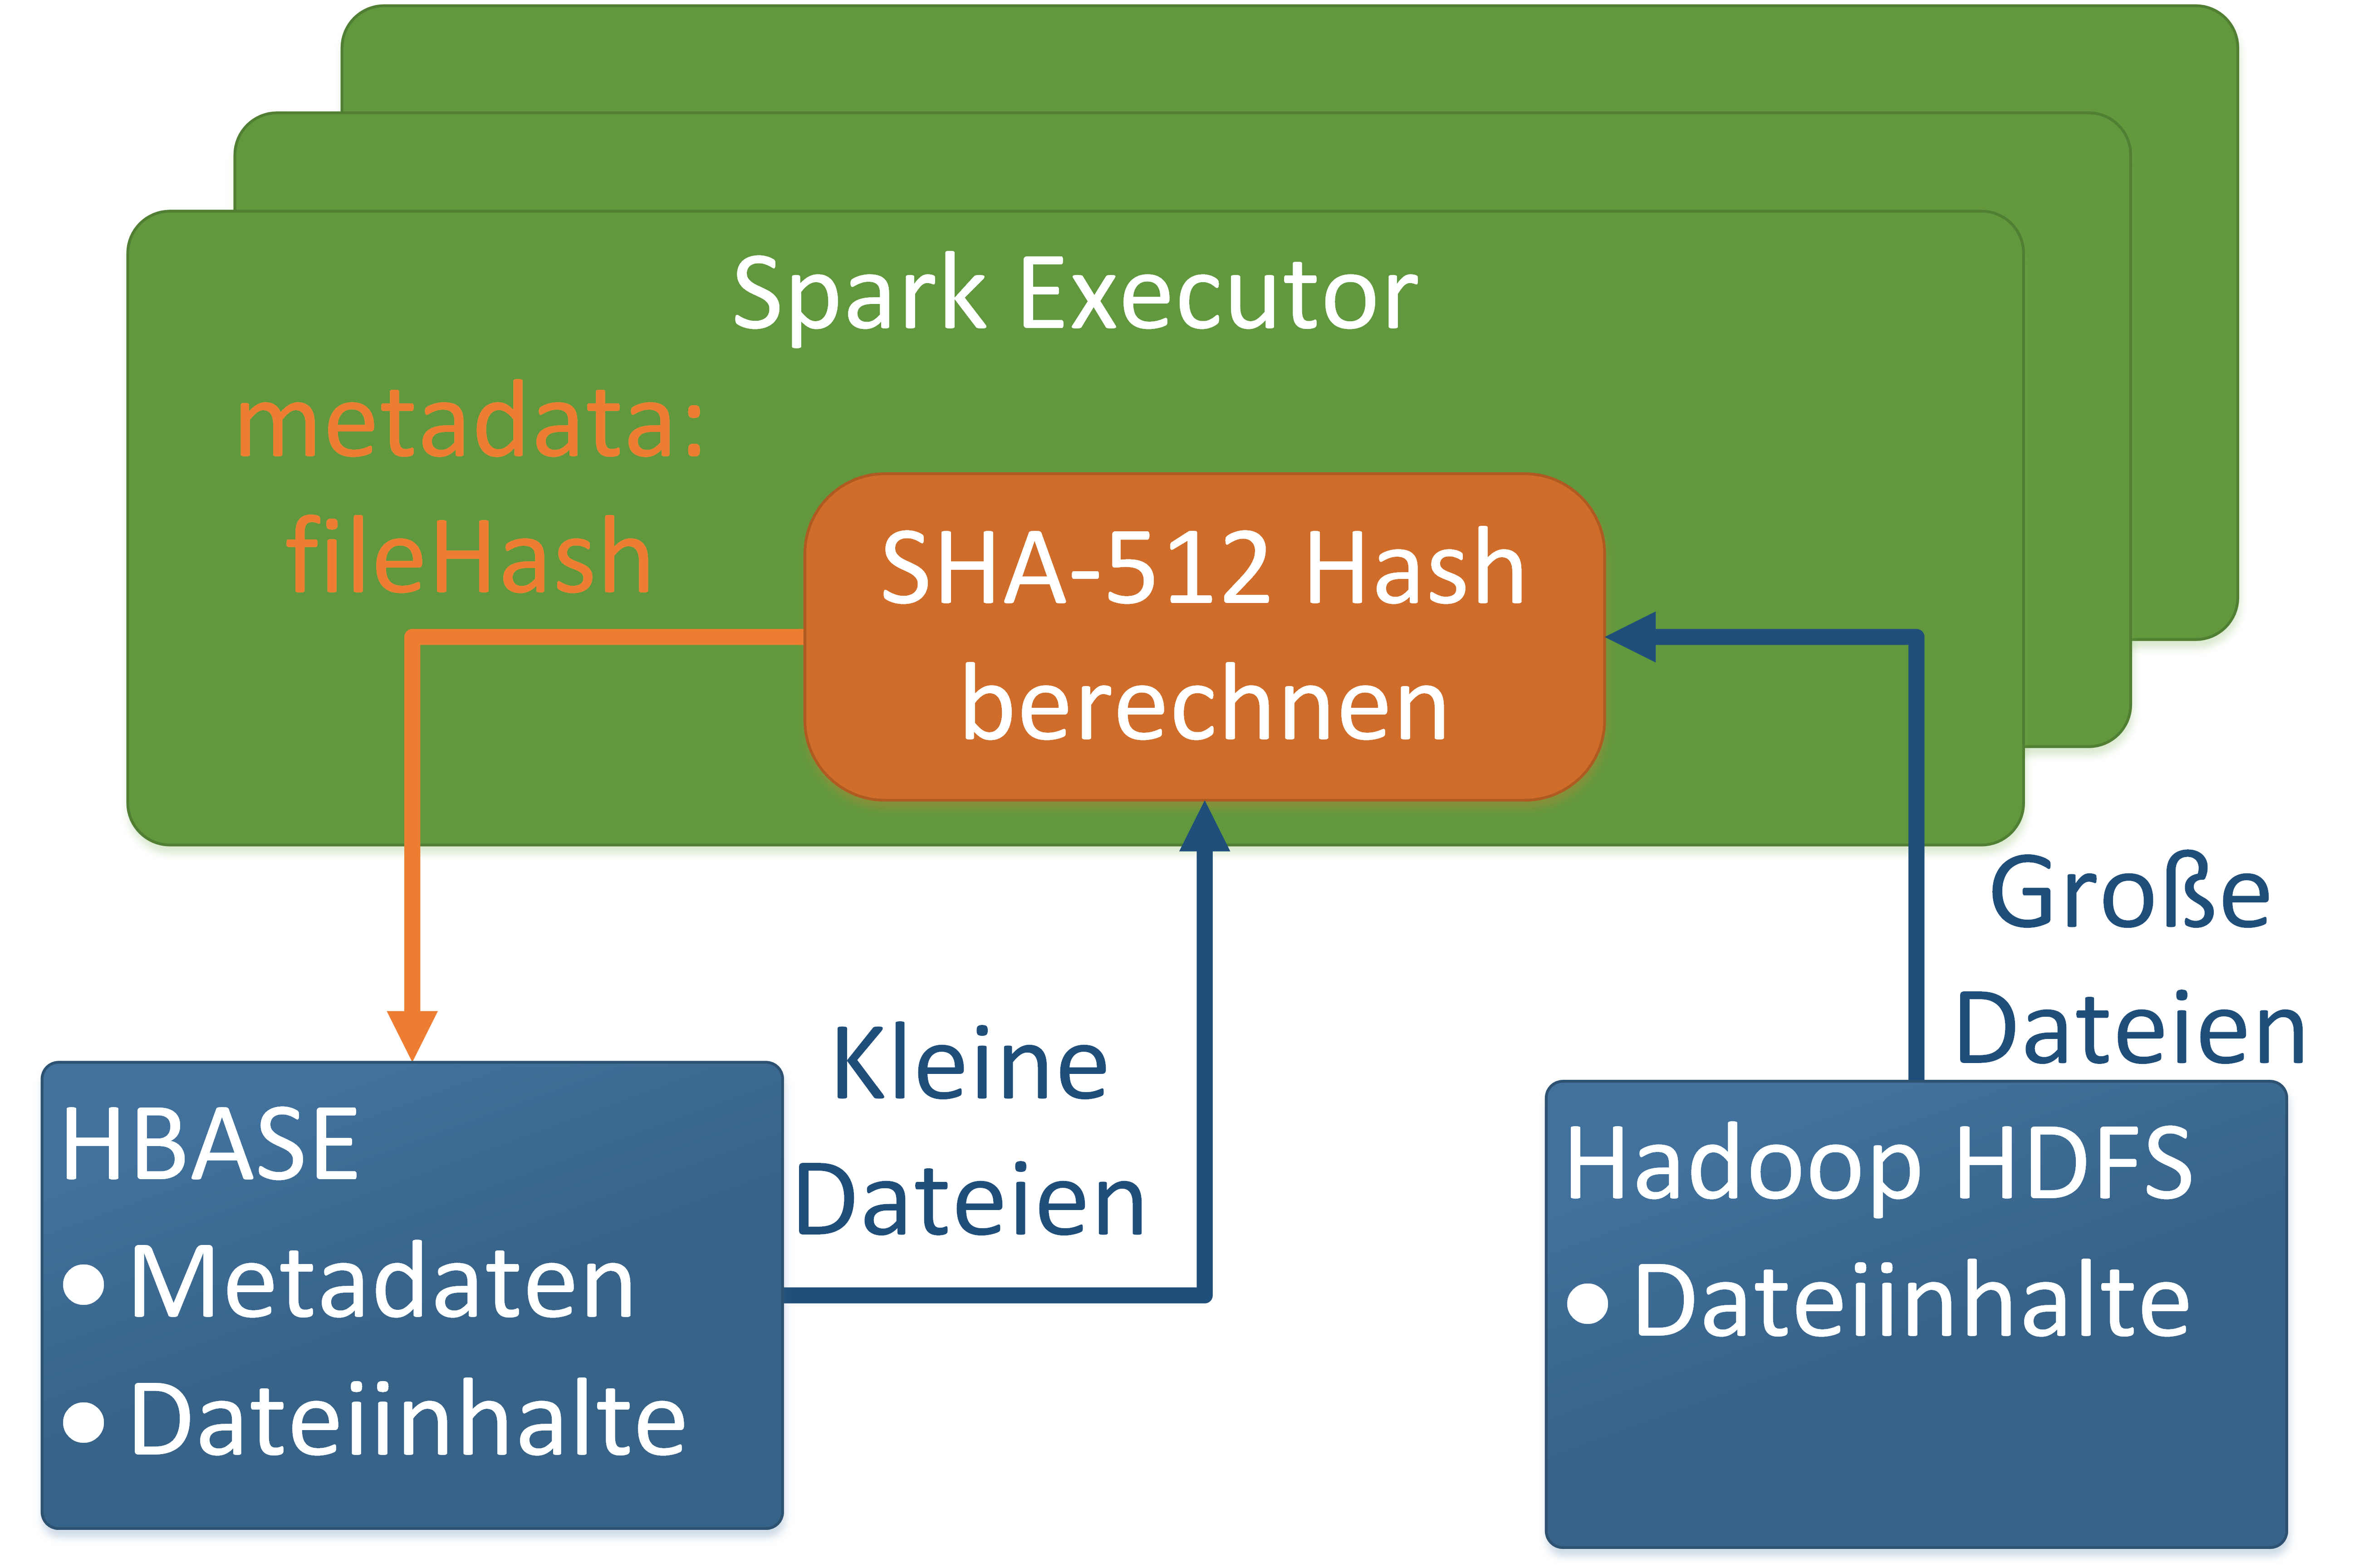
\includegraphics[width=0.78\textwidth]{./resource/spark_processing_hashes.png}
  \caption{Datenfluss bei der Berechnung von Hashsummen}
  \label{fig:data_processing_hashes}
\end{figure}

\noindent
Die Datenverarbeitung von kleinen Dateien aus HBASE und großen Dateien aus dem HDFS wird unabhängig voneinander in eigenen Spark-RDDs ausgeführt. Aufgrund der unterschiedlichen Datenquellen existieren auch zwei unterschiedliche Datentypen zum Auslesen der Dateiinhalte. Daher wird die Prozessierung in getrennten Tasks innerhalb der Spark Executoren ausgeführt. Um dann später die Hashsumme einer großen Datei aus dem HDFS in dem dazugehörigen Eintrag in HBASE abzuspeichern, ist es notwendig den Zeilenschlüssel des Eintrags in HBASE als Dateiname im HDFS zu verwenden. Dadurch können die Dateien aus dem HDFS einem Eintrag in HBASE zugeordnet werden.\\
Der ermittelte Hashwert wird darauf in der Spalte \textit{metadata:fileHash} in HBASE  gespeichert.\footnote{Siehe auch HBASE-Datenmodell in Abbildung \ref{fig:hbase_data_model}.}

\subsection{Duplikate erkennen}
\label{subsec:duplicate_files}
Aufbauend auf der Berechnung von Hashsummen können nun auch Datei-Duplikate ermittelt werden. Dadurch ist es möglich Beziehungen zwischen mehreren Asservaten herzustellen, wenn dort gleiche Dateien gefunden werden.\\
Derzeit werden diese Ergebnisse aber nur als Text im HDFS abgespeichert. In einer Weiterentwicklung könnten diese Informationen aber sehr gut in einer Graphendatenbank, wie beispielsweise \textit{Neo4j} abgespeichert werden. Hierdurch wäre visuell sehr schnell sichtbar, welche Beziehungen zwischen den Asservaten bestehen.\\ 
Allerdings wäre es in diesem Kontext dann auch sinnvoll, zwischen technischen Betriebssystemdateien und fachlichen Nutzerdateien zu unterscheiden. Denn wenn zwei Asservate das gleiche Betriebssystem enthalten, existieren auch zugleich tausende Datei-Duplikate. Interessant ist diese Erkennung von Duplikate aber gerade für fachliche Nutzerdaten, wie beispielsweise Bilder, Dokumente und Videos. Daran könnte später ermittelt werden, wie beispielsweise urheberrechtlich geschütztes Material über mehrere Systeme verbreitet wurde.\\

\noindent
Ein anderer Aspekt, welcher in einer Weiterentwicklung der Plattform implementiert werden könnte, ist der Vergleich mit bekannten Hashsummen von existierenden Datensätzen. Dies wird bei Autopsy verwendet, um gegebenenfalls Malware zu erkennen oder automatisiert nach spezifischen Dateien zu suchen. Ein Beispiel hierzu ist die sogenannte \textit{National Software Reference Library}, welche Hashsummen von bekannten Betriebssystem- und Anwendungsdateien enthält. Diese haben oftmals keinen forensischen Analysewert und könnten dann aus der Datenverarbeitung gefiltert werden.\footnote{Siehe Link: \url{https://www.nist.gov/itl/ssd/software-quality-group/nsrl-download/current-rds-hash-sets}. Letzter Zugriff: 9.9.2018.}\cite[S. 36]{digital_forensics}

\subsection{Medientypen erkennen}
\label{subsec:media_types}

Das Erkennen von Medientypen ist ein elementarer Bestandteil bei der Datenanalyse im Allgemeinen. Autopsy nutzt hierbei die Open-Source Bibliothek Apache Tika\texttrademark. Dieses Projekt wird auch in der forensischen Analyseplattform genutzt und ermittelt den Dateitype anhand des Dateiinhalts und der gegebenen Dateiendung.\\
Abbildung \ref{fig:data_processing_media_types} zeigt den Datenfluss bei der Ermittlung der Medientypen.\\

\begin{figure}[ht]
  \centering
  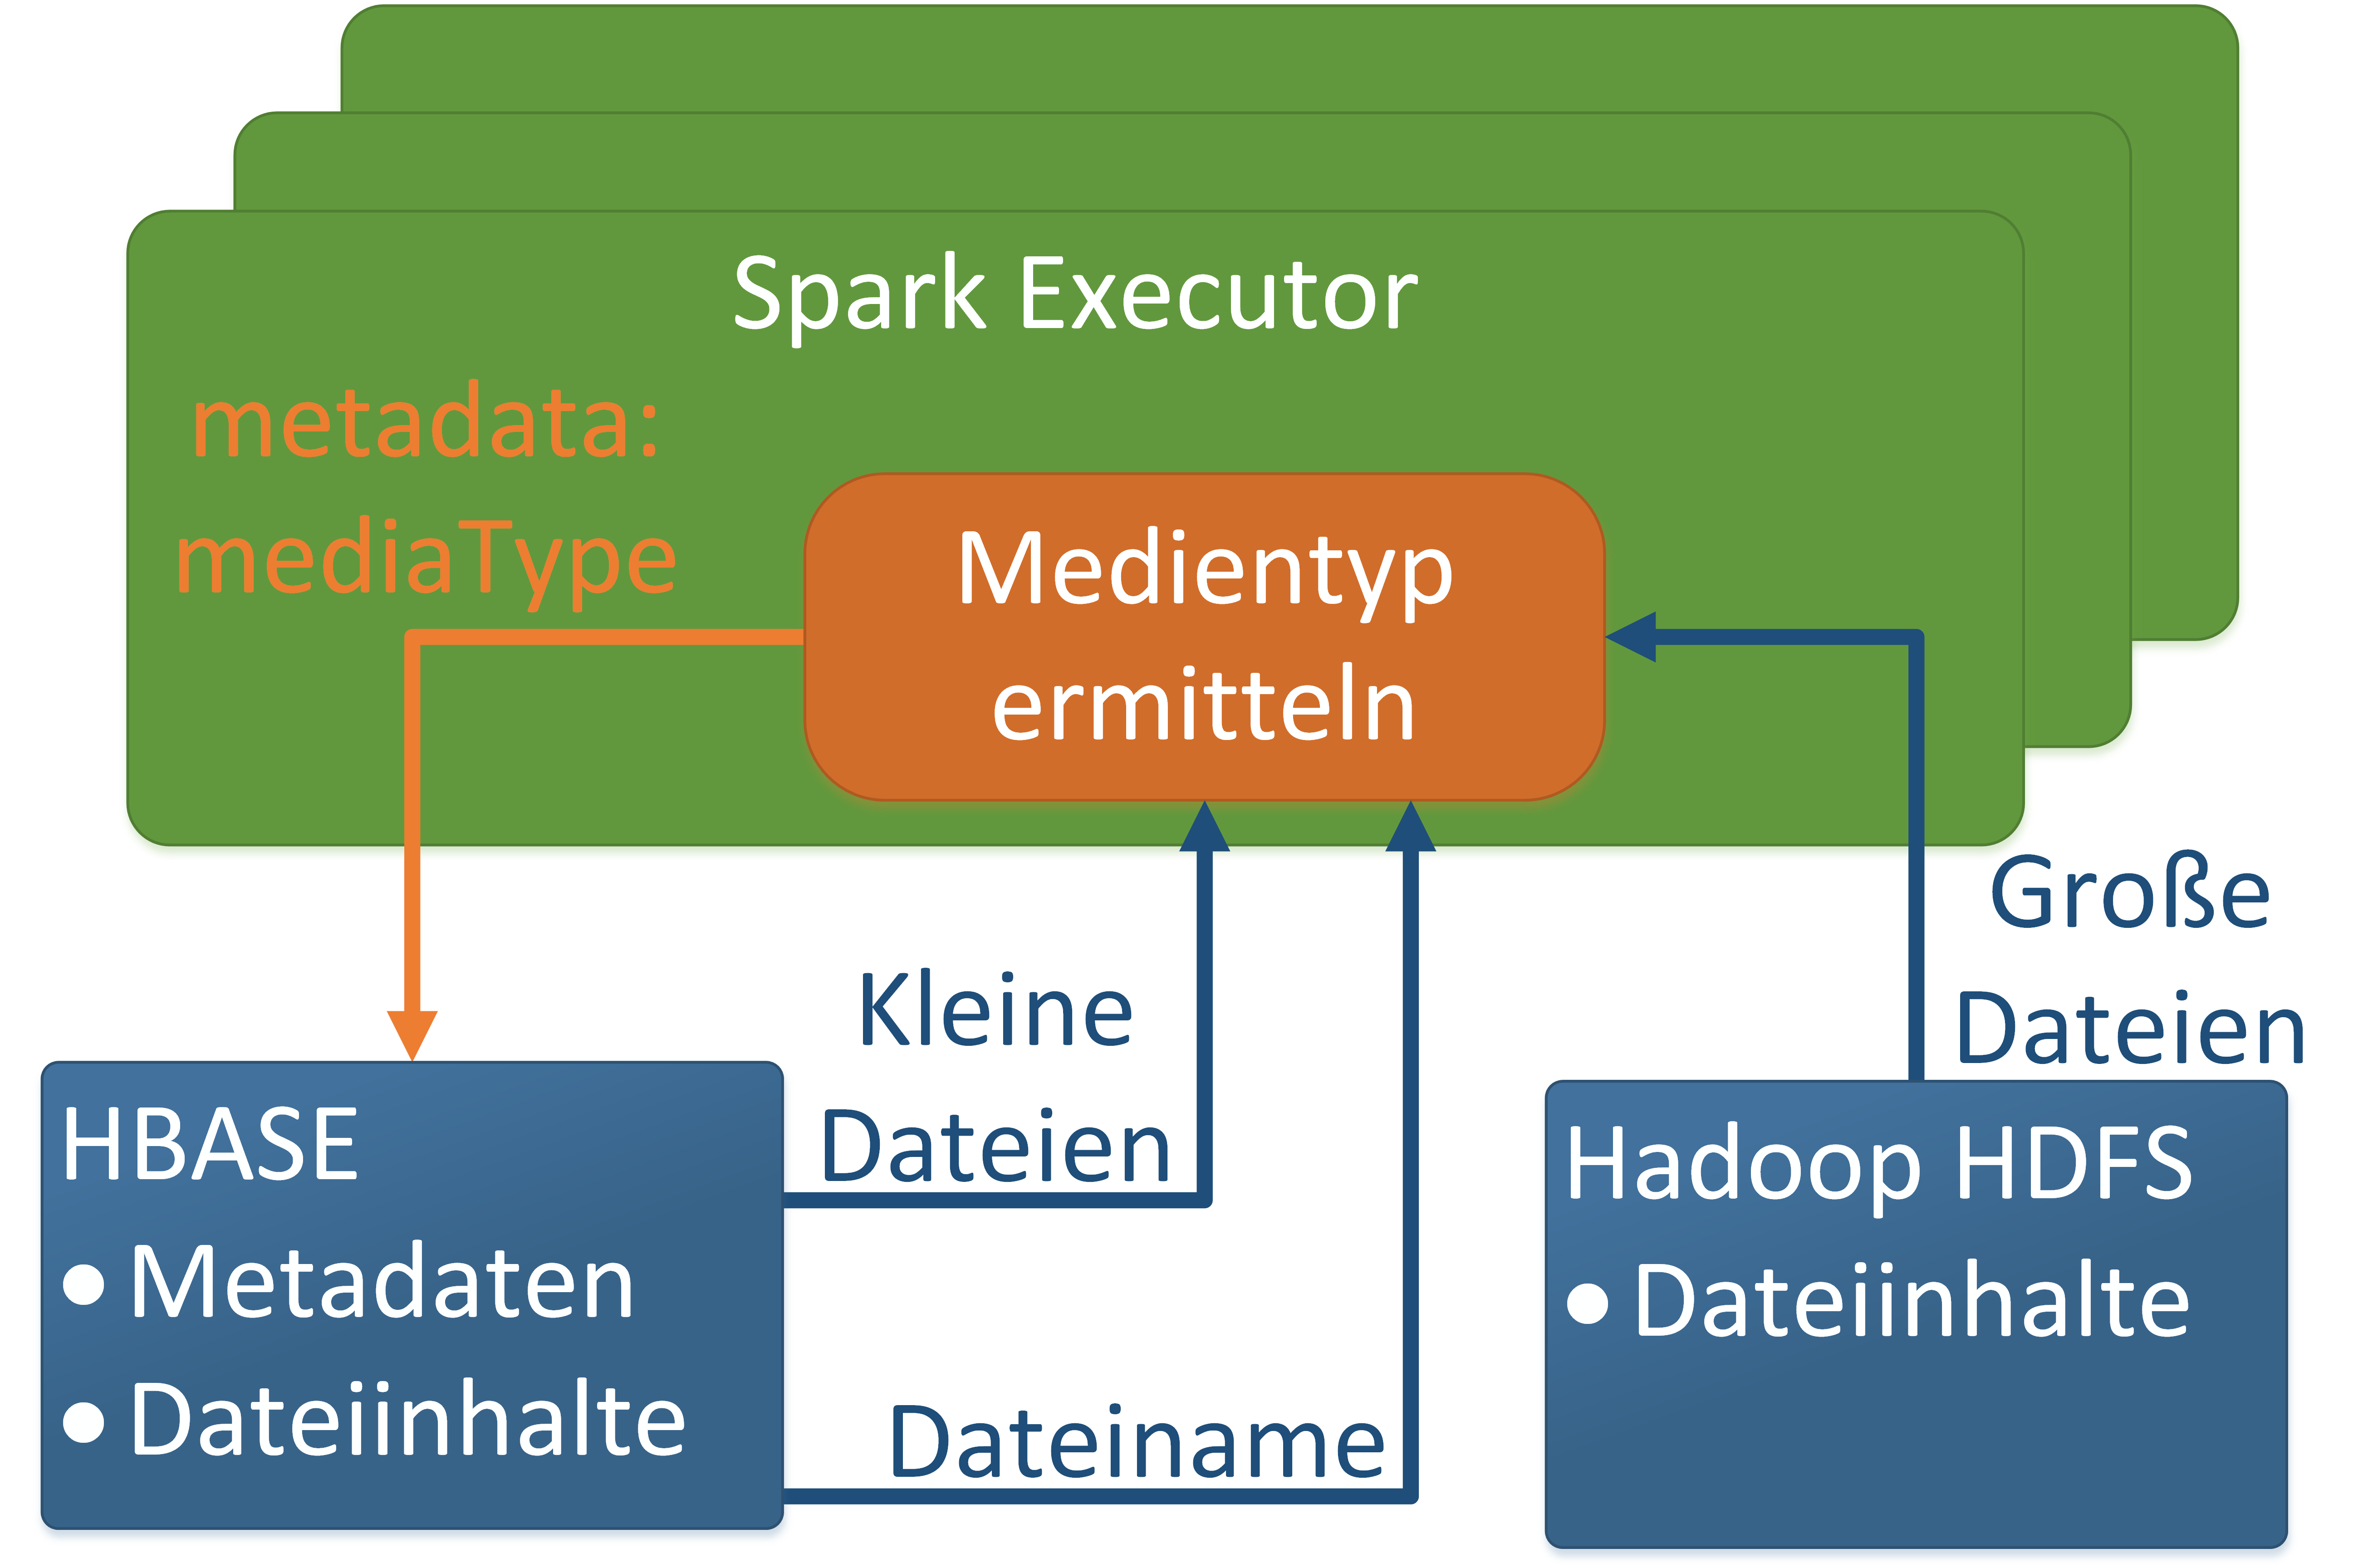
\includegraphics[width=0.78\textwidth]{./resource/spark_processing_media_types.png}
  \caption{Datenfluss bei der Ermittlung von Medientypen}
  \label{fig:data_processing_media_types}
\end{figure}

\noindent
Prinzipiell kann Apache Tika den Medientyp auch nur anhand der Dateiendung oder anhand des Dateiinhalts erkennen. Wird allerdings nur der die Dateiendung angegeben, so könnten beispielsweise Bilddateien mit gefälschten Dateiendung nicht korrekt erkannt werden. Wird hingegen nur der Dateiinhalt angegeben, so prüft Tika formatspezifische Bytesequencen, welche oftmals am Dateianfang stehen. Bei Textdateien hingegen, kann es nur identifizieren, dass es sich um eine Textdatei handeln könnte. Gerade bei Textdateien macht es Sinn, die Dateiendung in die Analyse mit aufzunehmen, um ein genaueres Ergebnis zu erhalten. Dadurch kann Tika beispielsweise ermitteln, ob es sich um eine CSV-Datei oder eine HTML-Datei handelt. Allerdings sollten diese Ergebnisse kritisch hinterfragt werden. Wie bereits erwähnt, könnte eine gefälschte Dateiendung mit Textdateien zu einem falschen Ergebnis führen.\\

\noindent
Das Ermitteln der Medientypen macht gerade bei der Datenvisualisierung Sinn, da damit schnell nach allen vorhanden Bildern oder Videos gesucht werden kann.\footnote{Siehe auch Kapitel \ref{ch:data_visualization}.}

\subsection{Volltextsuche und Datenindexierung}
\label{subsec:file_indexing}
Um auf die Daten in der forensischen Analyseplattform einfach zugreifen zu können, wäre eine Volltextsuche sinnvoll. Diese sollte performant arbeiten, damit Ergebnisse zu Suchanfragen von beliebigen Schlüsselwörtern in Realzeit angezeigt werden können. Um dies zu ermöglichen, können die Dateiinhalte und Metadaten indexiert werden.\\

\noindent 
Es gibt hierzu zwei mögliche Open-Source Projekte, die eine Datenindexierung anbieten. Dies sind \textit{Apache Solr\texttrademark} und Elasticsearch\texttrademark. Beide bieten eine Indexierung auf Basis von Apache Lucene an. Apache Solr wurde bereits im Grundlagenkapitel \ref{sec:theory_solr} beschrieben. Beide Projekte bieten einen ähnlichen Funktionsumfang. Im Rahmen dieser Thesis wird jedoch Apache Solr aus nachfolgenden Gründen genutzt.\\
Apache Solr bietet einen Cloud-Modus an und nutzt Apache Zookeeper, um die einzelnen Instanzen zu koordinieren. Für Apache Solr existiert bereits eine Integration in das Hadoop-Framework und die hier verwendete \textit{Hortonworks Data Platform}.\footnote{Siehe Link: \url{https://docs.hortonworks.com/HDPDocuments/HDPS/HDPS-3.0.0/bk_solr-search-installation/content/ch_hdp-search.html}. Letzter Stand: 9.9.2018.}\\
Elasticsearch bietet auch einen Cloud-Modus und ist horizontal skalierbar. Allerdings wird ein eigener Mechanismus dafür genutzt und es existiert für die \textit{Hortonworks Data Platform} kein Installationspaket zur Nutzung von Elasticsearch im Hadoop-Umfeld. Dies bedeutet, dass Elasticsearch eigenständig im Computer-Cluster ausgerollt und überwacht werden muss.\\
Ein weiterer Punkt ist die Absicherung der Cluster mithilfe von Kerberos. Prinzipiell können beider Projekte mit Kerberos abgesichert werden. Allerdings ist die Funktionalität bei Elasticsearch nur in einem kostenpflichtigen Zusatzpaket der Firma \textit{Elastic}\footnote{Siehe Link: \url{https://www.elastic.co/}. Letzter Stand: 9.9.2018.} enthalten.\\
Zuletzt unterscheiden sich beide Projekte auch in der Art und Weise, wie die Daten verteilt indexiert werden können. Bei Elasticsearch gibt es eine Bibliothek, welche die bereits bekannten \textit{Apache Spark Resilient Distributed Datasets} (RDDs) direkt in Elasticsearch indexieren kann.\footnote{Siehe Link: \url{https://www.elastic.co/guide/en/elasticsearch/hadoop/current/spark.html}. Letzter Stand: 9.9.2018.} Diese Möglichkeit ist prinzipiell sehr gut, um extrahierte Daten direkt indexieren zu können.\\
Apache Solr hingegen bietet auch eine Möglichkeit mit Apache Spark Daten in die Solr-Cloud zu indexieren.\footnote{Siehe Link: \url{https://github.com/lucidworks/spark-solr}. Letzter Stand: 9.9.2018} Allerdings ist die Schnittstelle etwas umständlicher nutzbar, da keine RDDs sondern die bereits beschriebenen \textit{DateFrames} genutzt werden müssen.\\
Viel interessanter ist jedoch das Open-Source Projekt \textit{Lily HBase Indexer}.\footnote{Siehe Link: \url{https://github.com/NGDATA/hbase-indexer}. Letzter Stand: 9.9.2018.} Damit können Daten direkt aus HBASE in den Solr-Cluster indexiert werden. 
Im Rahmen der Thesis wird letztes Projekt genutzt, um die Metadaten aus HBASE in Solr zu indexieren. 




Ein weitere Anwendungsfall ist die Indizierung von Texten und Wörtern, welche aus den einzelnen Dateien extrahiert wurden.\\

\noindent
Der Grund für eine Indizierung dieser Inhalte ist eine schnellere Suche nach beliebigen Wörtern, als bei der reinen Suche in HBASE. Zur Indizierung existieren zwei bekannte Projekt. Diese sind einerseits \textit{Apache Solr} und andererseits \textit{Elasticsearch}. Bei bauen wiederum auf das \textit{Apache Lucene}-Projekt auf. Apache Solr ist ein Open-Source Projekt unter dem Dach der Apache Foundation. Wohingegen Elasticsearch auch als Open-Source Projekt entwickelt wird, jedoch primär von der kommerziellen Firma \textit{Elastic???} verwaltet wird. Diese bietet gerade Zusatzpakete und Support gegen Bezahlung an.
Siehe auch \cite[S.7]{solr_search}
\subsubsection{Apache Solr}
Spark-Connector von Databracks vorhanden. Der Connector selbst bietet aber vorzugsweise lesenden Zugriff.

\noindent
Abbildung \ref{fig:hbase_solr_indexing} stellt die physikalische Aufteilung mit dem hbase-indexer projekt

\begin{figure}[ht]
  \centering
  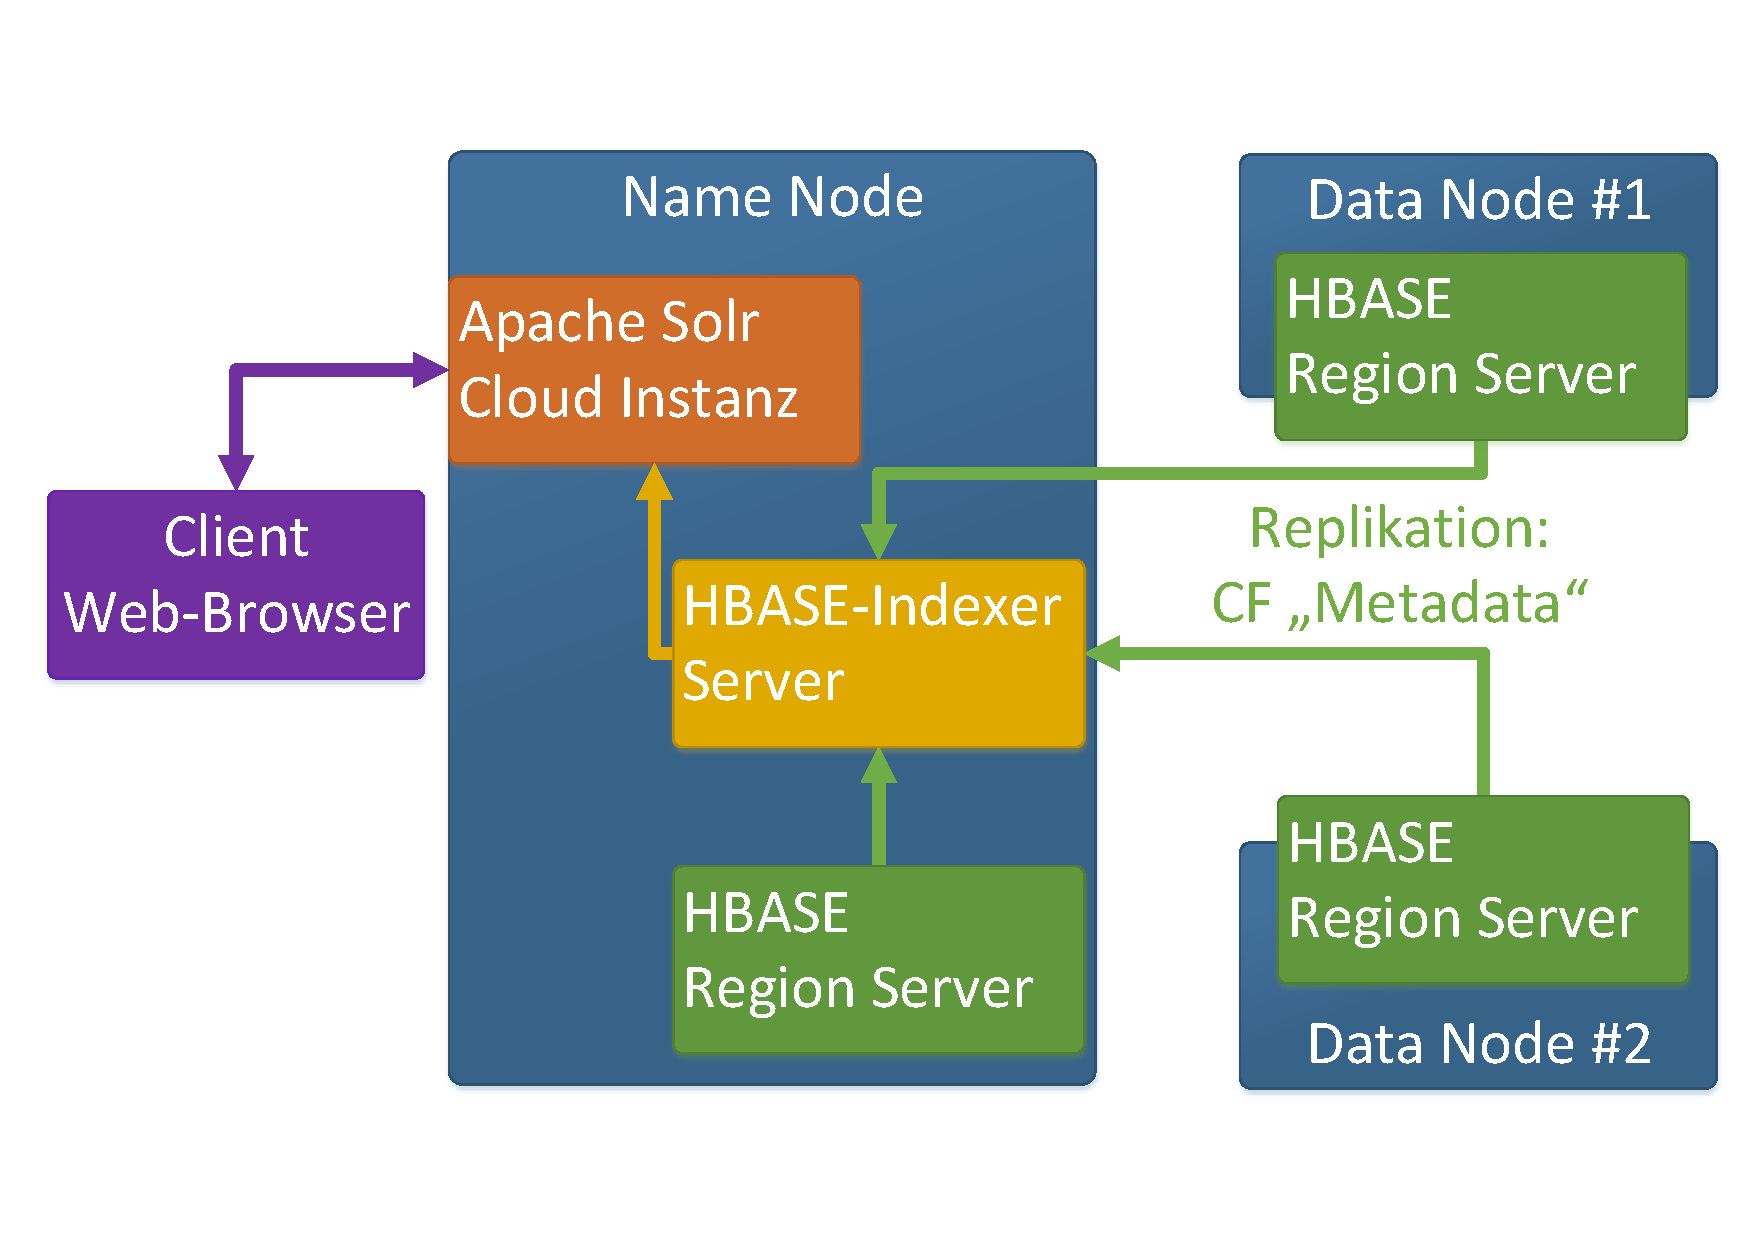
\includegraphics[width=\textwidth]{./resource/hbase_solr_indexierung.pdf}
  \caption{Indexierung von Daten aus HBASE in Solr}
  \label{fig:hbase_solr_indexing}
\end{figure}

%TODO : Vergleich zu Elasticsearch!
%Spark-Connector auf RDD-Basis vorhanden. Kerberos-Sicherung nur über X-Pack gegen Geld vorhanden. Rack-Awareness und Verteilung nicht klar. Elasticsearch baut eigene Infrastruktur auf. Nicht über Ambari steuerbar.

\section{Praxisbeispiele und deren Optimierungen}
Gerade bei der Verarbeitung großer Datenmengen und unter Berücksichtigung des Prinzips der Datenlokalität existieren einige Fallstricke und Hürden bei der Implementierung der Datenverarbeitung. Im Hadoop-Umfeld und bei der Entwicklung im Spark-Context geht es nicht nur um die Art und Weise, wie die Algorithmen auf die Daten angewendet werden, sondern in erster Linie auch immer darum \textbf{wo} die einzelnen Programmteile ausgeführt werden. 
Der Entwickler sollte immer wissen, in welchem Verarbeitungskontext er sich befindet. Zu dieser Problematik werden in diesem Kapitel einige Beispiele herausgegriffen, welche während der Bearbeitung dieser Thesis aufgetreten sind.\\

\noindent
\subsection*{Weniger ist mehr TODO}
Ungenutzte Daten so früh wie möglich aus der Verarbeitung rausnehmen. Siehe
Problematik beim HBASE-Spark Connector. Entweder ich mache einen Full-Table Scan und fodere
alle Daten an, um sie später im Spark-Executor auszuführen, oder ich versuche schon beim Zugriff der Daten in den Region-Server mit ColumnFamilies und Filter-Operationen nur die Daten anzufordern, welche auch wirklich benötigt werden. 
\subsection*{Caching - Performanz vs. Ressourcen TODO}
Hashing-Problem. Ist es geschickter Daten zu Cachen anstatt sie zweifach anzufordern?
Funktioniert Caching überhaupt mit nicht serializierbaren Daten?
\subsection*{Faulheit ist der Schlüssel zum Erfolg TODO}
Lazy-Loading und Ausführung bei RDDs

\subsection*{Teile und Herrsche TODO}
Balancing and Repartitionieren. Aufteilung der Last zu gleichen Teilen!
Gerade beim Ausprobieren und Testen ist es einfach, die Resultate eines RDDs nach der Datenverarbeitung über eine Konsole auszugeben. Doch hierbei muss genau überlegt werden, wie diese Resultate ausgegeben werden (siehe Listing \ref{lst:spark_rdd_collect}). In der ersten Variante wird auf dem RDD die Methode collect() aufgerufen und die daraus erhaltene Liste von Objekten wird über ein Logger-Objekt in das Log-File dieser Ausführung geschrieben.\\
Auf der ersten Blick ist aber nicht ersichtlich, was diese Methode wirklich bewirkt. Wie bereits in Kapitel \ref{sec:theory_spark} (TODO: check reference) beschrieben, wird bei der Ausführung einer Spark-Anwendung ein sogenannter Spark-Driver gestartet. Dieser wiederum fordert eine gewisse Anzahl von Exekutoren an, die die eigentlich Datenverarbeitung übernehmen (Master-Slave-Prinzip). Hierbei laufen die Executoren auf einzelnen Knoten innerhalb des Clusters. In dem Moment, in welchem die collect()-Methode auf einem RDD ausgeführt wird, werden die Daten des RDDs \textit{eingesammelt}. Dies bedeutet, dass die Daten des RDDs, welche vorher verteilt auf allen Executoren im Arbeitsspeicher geladen wurden, nun jetzt an den Spark-Driver geschickt werden. Dieser sammelt sozusagen die Ergebnisse der Executoren ein. Diese Mechanismus ist an sich nicht problematisch und funktioniert auch gerade beim Testen mit kleinen Datenmengen. Bei großen RDDs hingegen, werden auch wieder alle Daten an der Driver geschickt und in den meisten Fällen wird dies den begrenzten Arbeitsspeicher des Drivers überfordern. Die Applikation wird mit einer OutOfMemoryException??? beendet!.\\

\noindent
Daher ist es sinnvoll auch schon beim Testen mit kleinen RDDs vorzugsweise die take()-Methode zu nutzen. Diese tut das gleiche wie, die collect()-Methode mit dem Zusatz, dass sie nur ein bestimmte Anzahl von Einträgen sammelt. Dadurch wird selbst bei größeren RDDs der Speicher nicht ausgehen. 


\begin{lstlisting}[label={lst:spark_rdd_collect},caption= Spark Java RDD collect()-Methode ,captionpos=b,frame=single,style=customjava]

HbaseReader hbr = new HbaseReader(jsc, hbaseConfigFile);
JavaRDD<Metadata> forensicMetadata = hbr.getForensicMetadata();

// use collect() method
forensicMetadata.collect().stream()
	.forEach(m -> LOGGER.info("Entry = .", m));

// use take(int amount) method	
forensicMetadata.take(10).stream()
	.forEach(m -> LOGGER.info("Entry = .", m));	
\end{lstlisting}

\section{Leistungsanalyse}
TODO: Geschwindigkeit und Ressourcenverbrauch analysieren. Hierzu gehört auch die Performanz beim Datenimport! Maximal 3 Seiten.

